\section{Mono-domain Equations with the Minimal Ventricular Model}

\newpage


\newpage
\section{Numerical Examples}


\subsection{A Single Cell Simulation}

A \textsl{semi-implicit} euler squeme can be apply to the system of equations (\ref{eq:mde_min}), neglecting the diffusion term, where all the non-linear terms are left explicit, while the linear ones are left implicit. This last simplify the problem cause linearise it. Also, note that with this squeme the system is un-coupled. Now, consider the following factorization for the discretized currents $\overline{J_{so}}$, $\overline{J_{si}}$ and $\overline{J_{fi}}$:

\begin{equation}
\arraycolsep=1.4pt\def\arraystretch{1.5}
\begin{array}{lr}
\overline{J_{so}} = & J_{so}^I \phi^{n+1} + J_{so}^E \\
\overline{J_{si}} = & J_{si}^E \\
\overline{J_{fi}} = & J_{fi}^I \phi^{n+1} + J_{fi}^E
\end{array} \label{eq:current_factorization}
\end{equation}

the potential and the gating variables for the $(n+1)$-time step can be calculated as follows:

\begin{equation}
\arraycolsep=1.4pt\def\arraystretch{2.8}
\begin{array}{l}
\phi^{n + 1} =  \dfrac{\phi^n - \Delta t (J_{fi}^E + J_{so}^E + J_{si}^E)}{1 + \Delta t (J_{fi}^I + J_{so}^I)} \\ 

r^{n+1} = \dfrac{r^n + (\Delta t r_{\infty}(1 - H(\phi - \theta_r)))/\tau_r^-}{1  +  (\Delta t (1 - H(\phi^n - \theta_r)))/\tau_r^- + (\Delta t H(\phi^n - \theta_r))/\tau_r^+} \\

w^{n+1} = \dfrac{w^n + (\Delta t w_{\infty}(1 - H(\phi - \theta_w)))/\tau_w^-}{1  +  (\Delta t (1 - H(\phi^n - \theta_w)))/\tau_w^- + (\Delta t H(\phi^n - \theta_w))/\tau_w^+} \\
   
s^{n+1} = \dfrac{s^n + \Delta t (1 + tanh(k_s (\phi^n - \phi_s)))/(2 \tau_s)}{(1 + \Delta t / \tau_s)}
\end{array} \label{eq:mde_min_imp}
\end{equation}

The dimensionless voltage variable is re-scaled to obtain values inside the physiological range, with the equation $\phi_{mV} = 85.7 \phi - 84$ or with  $\phi_{mV} = 85.7 \phi - 80.9$ if the tissue if from the atrial chamber. The initial scaled conditions are $\phi = 0$, $r = 1$, $w = 1$ and $s = 0$. To ``move'' the cell from the rest state, a stimulus of $52 [mV]$ is applied for $0.2 [ms]$, in order to reproduce the $Na^+$ channels overture, i.e., the transition to phase 1. Note that this value is over the threshold needed to generate the action potential\footnote{Note that this physiological property cannot be emulated with the FitzHugh-Nagumo model.} of the cell. \\

A time-step of $0.1 [ms]$ is used. The result of the implementation can be seen in the figure \ref{fig:mde_min_ex1_single-cell}.

\begin{figure}[H]
\centering
\subfigure[epicardial cell.]{
	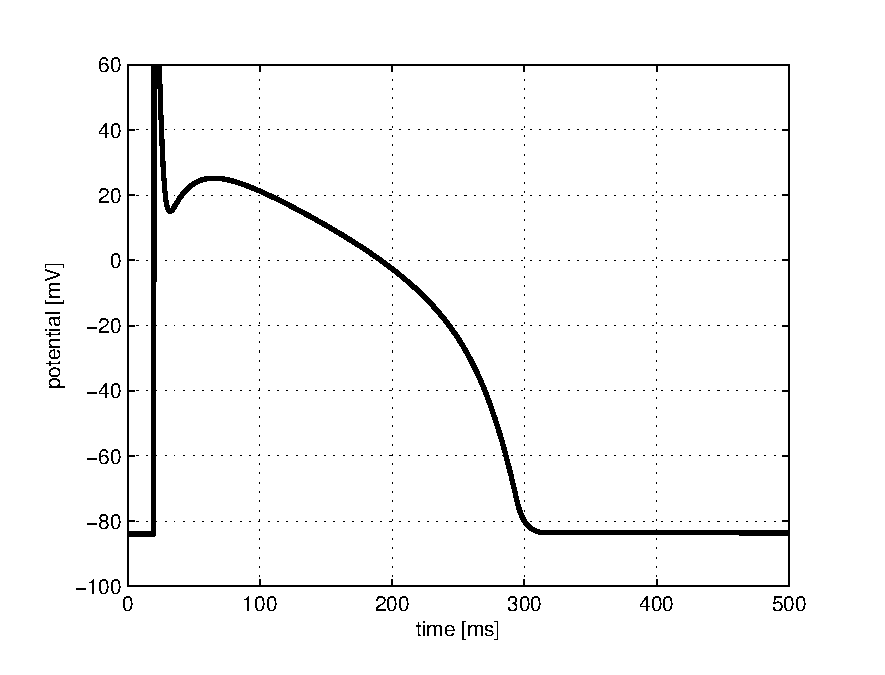
\includegraphics[height = 2.5 cm]{fig/mde_min_ex1_single-cell_epi}}
\subfigure[endocardial cell.]{
	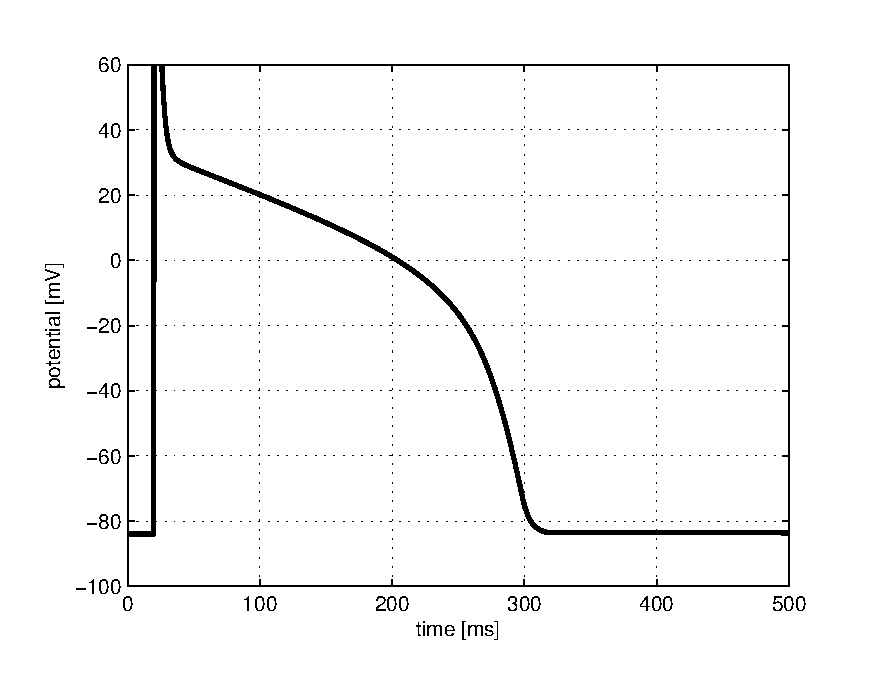
\includegraphics[height = 2.5 cm]{fig/mde_min_ex1_single-cell_endo}}
\subfigure[mid-myocardial cell.]{
	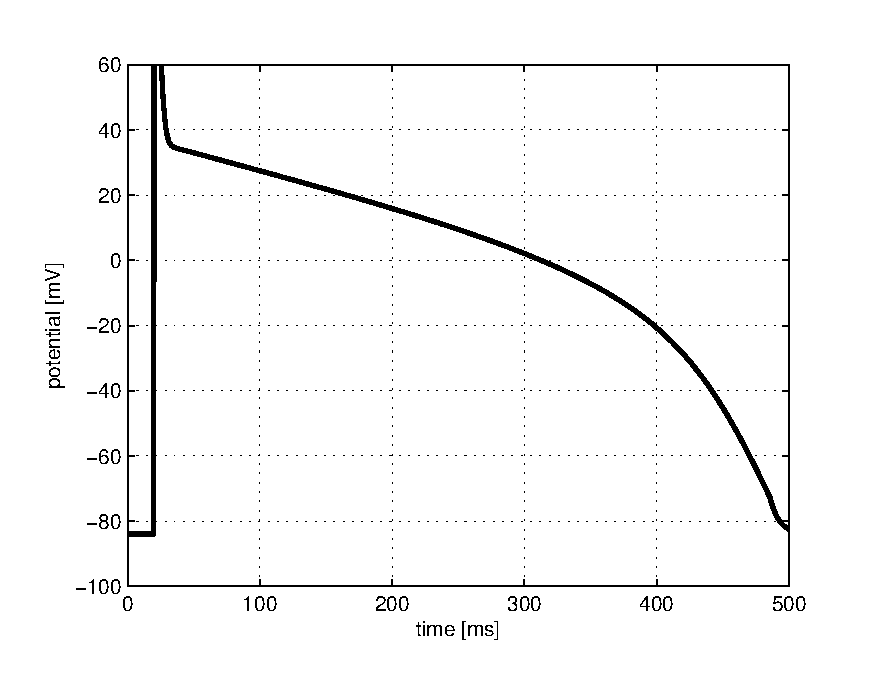
\includegraphics[height = 2.5 cm]{fig/mde_min_ex1_single-cell_mid}}
\subfigure[atrial cell.]{
	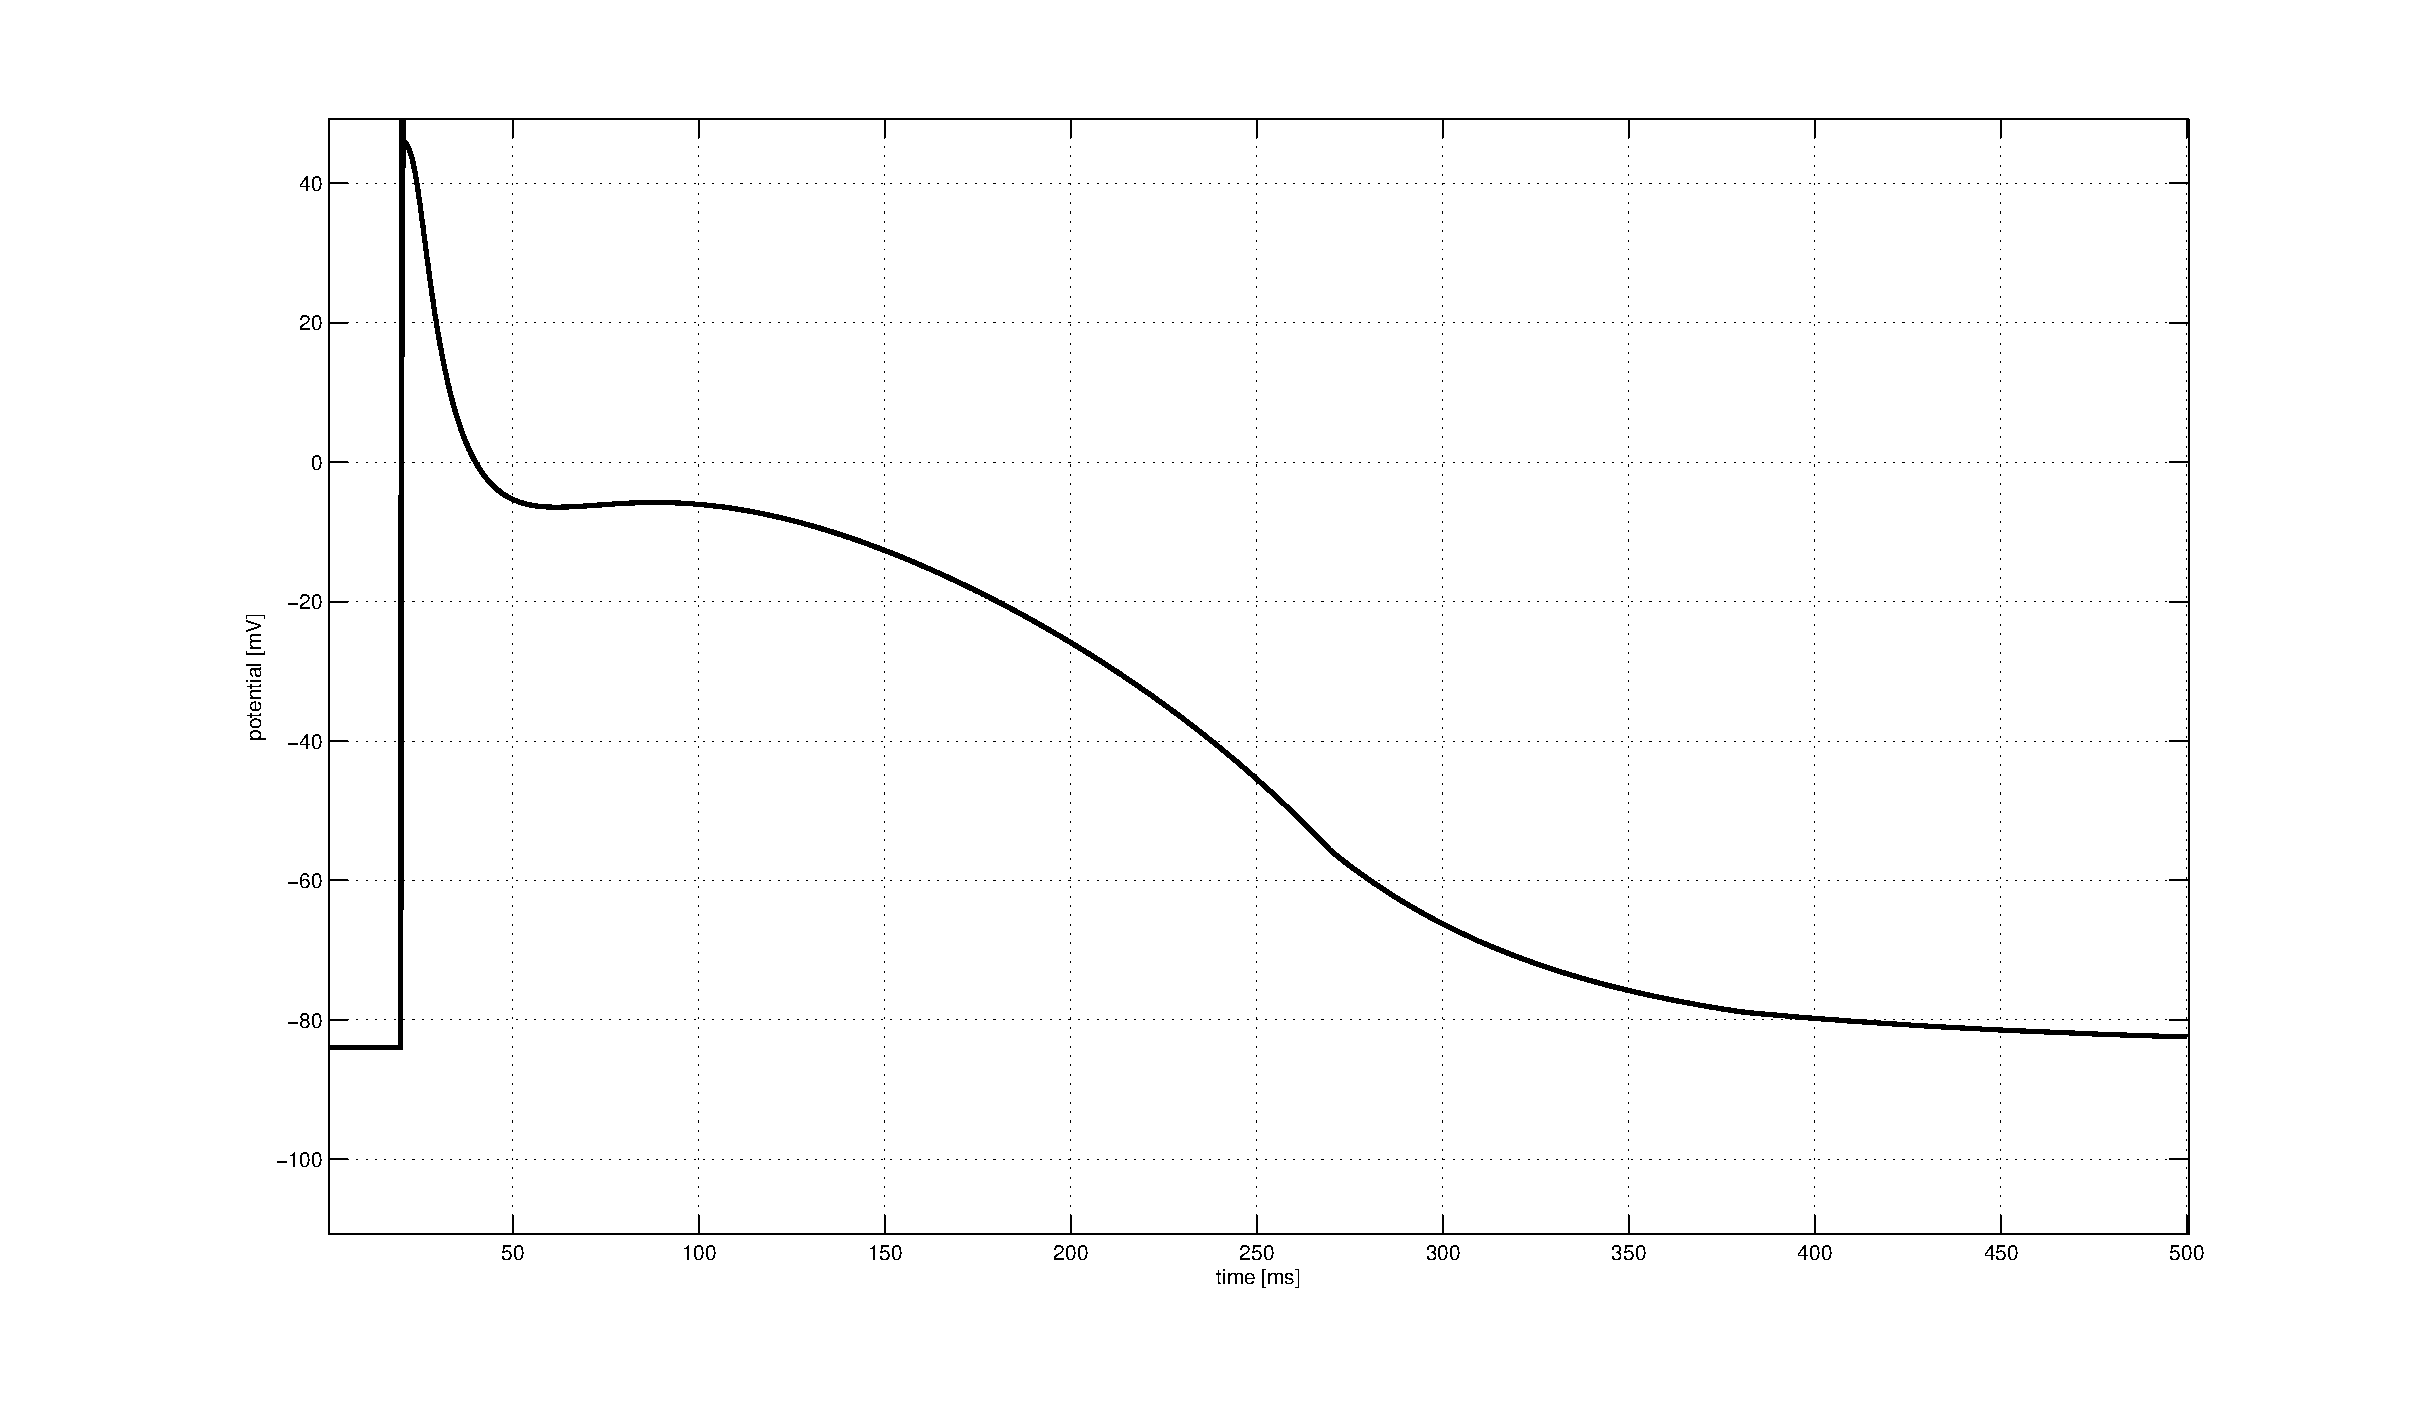
\includegraphics[height = 2.5 cm]{fig/mde_min_ex1_single-cell_atrial}}
\caption{simulated human AP for different configurations.} \label{fig:mde_min_ex1_single-cell}
\end{figure}

\newpage 
\subsection{A Non-Fibrotic Tissue Simulation}

Now consider a non-fibrotic epicardial tissue, and the configuration of the table (\ref{tab:mde_min_setup_1}). A stimulus is applied in the left edge from 0 to 2 ms in simulation time.

\begin{table}[H]
\centering
\begin{tabular}{@{}lr@{}}
\toprule
\multicolumn{1}{c}{Parameter} & \multicolumn{1}{c}{Set-Up}                                            \\ \midrule
Domain                        & $[0, 25] \times [0, 25] mm^2$ square                                    \\
Boundary Conditions           & $\partial_x \phi = 1.587 \delta, \forall \vec{x} \in \partial \Omega$ \\
Initial Conditions            & $\phi = 0$, $r = 1$, $w = 1$ and $s = 0$, $\forall \vec{x} \in \Omega$             \\
DOF's       & 809405                                                                    \\
$d_1$						 &   0.154 $[mm^2/ms]$ \\
$\theta_c$                    & 0                                                                   \\
$\gamma$                      & 4                                                                     \\
$\Delta t $                  & 0.1 [ms]                                                                 \\
Total time & 500 [ms] \\ \bottomrule
\end{tabular}
\caption{setup for experiment.} \label{tab:mde_min_setup_1}
\end{table}

where, for $x = (x_1, x_2) \in \Omega$, $\delta$ is defined as follows:

\begin{equation}
\delta = \left\lbrace \begin{array}{cc}
1 & \text{ if }  \{ 0 [ms] < t < 2 [ms] \wedge x_1 = 0  \} \\
0 & \text{ i.o.c }
\end{array} \right.
\end{equation}

For the details about the discretization (in both, time and space) for this and the following experiments, see appendix (1). The result of the implementation is shown in figure \ref{fig:results_exp1}.

\begin{figure}[H]
\centering
\subfigure{
	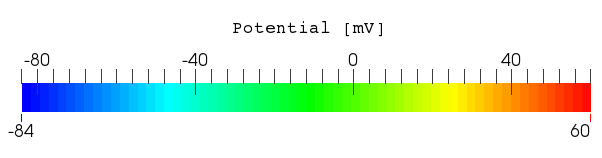
\includegraphics[height = 1.5 cm]{fig/numerical_example_mde+min_exp1_colourbar}
	} \\
\subfigure[0 ms]{
	
\includegraphics[height = 3 cm]{fig/numerical_example_mde+min_exp1_0ms}
	}
\subfigure[3 ms]{
	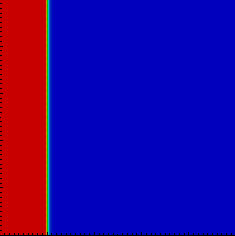
\includegraphics[height = 3 cm]{fig/numerical_example_mde+min_exp1_3ms}
	}	
\subfigure[10 ms]{
	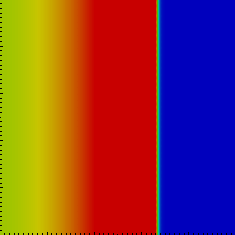
\includegraphics[height = 3 cm]{fig/numerical_example_mde+min_exp1_10ms}
	}
\subfigure[20 ms]{
	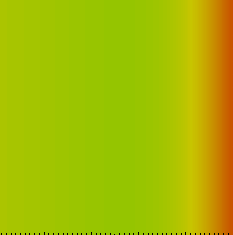
\includegraphics[height = 3 cm]{fig/numerical_example_mde+min_exp1_20ms}
	}
\subfigure[150 ms]{
	
\includegraphics[height = 3 cm]{fig/numerical_example_mde+min_exp1_150ms}
	}
\subfigure[250 ms]{
	
\includegraphics[height = 3 cm]{fig/numerical_example_mde+min_exp1_250ms}
	}
\subfigure[350 ms]{
	
\includegraphics[height = 3 cm]{fig/numerical_example_mde+min_exp1_350ms}
	}
\caption{evolution of the potential over the tissue.} \label{fig:results_exp1}
\end{figure}

In the figure \ref{fig:results_exp1_2points} the temporal evolution of the potential for two aislated points can be seen, one in the point (12.5, 12.5) and the other in the point (25, 12.5).

\begin{figure}[H]
\centering
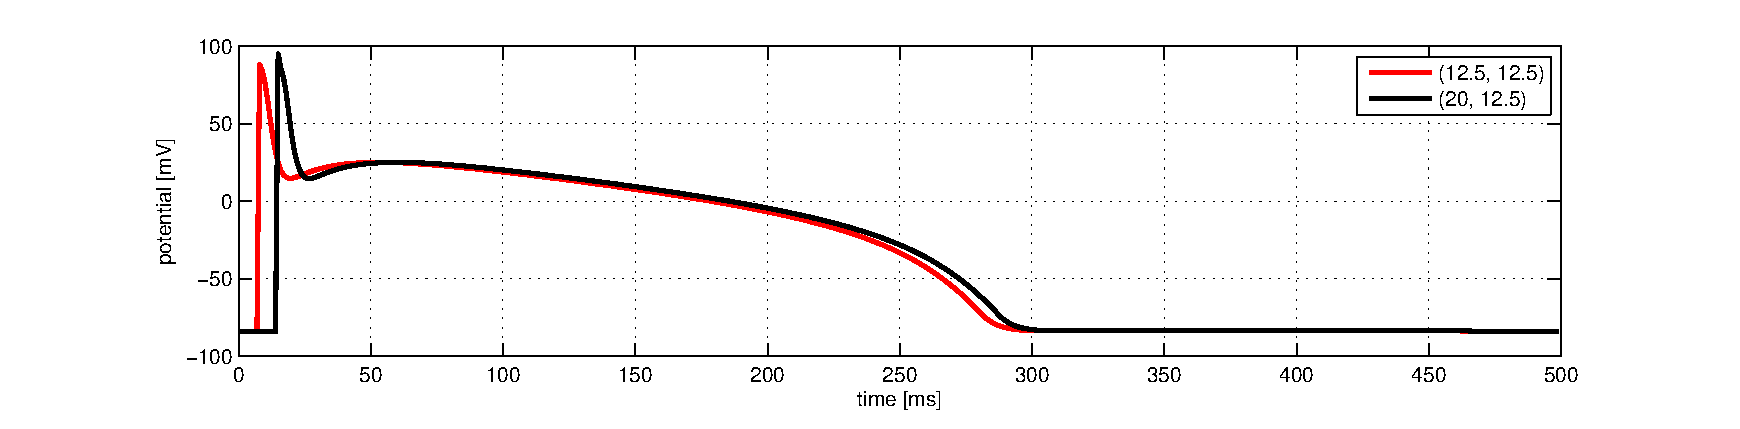
\includegraphics[height = 4 cm]{fig/numerical_example_mde+min_exp1_point1}
\caption{action potential evolution for two separated points.} \label{fig:results_exp1_2points}
\end{figure}

The domain in study is large enough (todo: citar panfilov) to perform a study of the CV of the tissue. So, comparing the peaks of both points, the conduction velocity is calculated and gives a value of 1.78 [mm/ms], which is a physiological accepted value.

\newpage 
\subsection{A Tissue with Diffuse Fibrosis Simulation}

On this experiment, a endocardial tissue with diffuse fibrosis will be simulated. To do this, a rank-2 homogenizations will be done, and both problems, exact and homogenized, will be compared. Lets consider the configuration of the table \ref{tab:mde_min_setup_2}. \\

\begin{table}[H]
\centering
\begin{tabular}{@{}lr@{}}
\toprule
\multicolumn{1}{c}{Parameter} & \multicolumn{1}{c}{Set-Up}                                            \\ \midrule
Domain                        & $[0, 25] \times [0, 25] mm^2$ square                                    \\
Boundary Conditions           & $\partial_x \phi = 1.587 \delta, \forall \vec{x} \in \partial \Omega$  \\
Initial Conditions            & $\phi = 0$, $r = 1$, $w = 1$ and $s = 0$, $\forall \vec{x} \in \Omega$             \\
DOF's for Exact Problem       &    1209500                                                               \\
DOF's for Homogenized Pb.     &       81900                                                               \\
a &	0.1[mm] \\
b & 1 [mm] \\
$d_1$						 & \red{0.154 si el valor de CV da muy grande}  0.1171 $[mm^2/ms]$ \\
$\theta_c$                    & 0.4                                                                   \\
$\theta_f$                    & 0.5                                                                   \\
$\beta$                       & $10^{-5}$                                                             \\
$\gamma$                      & 4                                                                     \\
$\Delta t $                  & 0.1 [ms]                                                                \\
Total Time					& 500 [ms]
 \\ \bottomrule
\end{tabular}
\caption{setup for experiment.} \label{tab:mde_min_setup_2}
\end{table}

In the figure \ref{fig:subdomains_R2} the configuration and a zoom of the mesh used is shown. Also, the mesh used for the homogenized problem is presented in the figure \ref{fig:mesh_h}. The external stimulus are similar to experiment (2).

\begin{figure}[H]   
\centering
\includegraphics[height = 5 cm]{fig/malla_exp2}
\caption{ a fraction of the domain (the entire domain has 25 collagen incrustation per side) in study for diffuse fibrosis (left) and a zoom of the mesh to solve the exact problem (right).} \label{fig:subdomains_R2}
\end{figure}

The mesh for the exact problem has a characteristic triangle size of 10 $[\mu m]$ near the collagen, and of 0.15 [mm] in the rest of the domain, while the coarse mesh for the homogenized problem has a characteristic size of 0.15 [mm] over all the domain. 

The result of the implementation is presented in the figure \ref{fig:results_exp2}.

\begin{figure}[H]
\centering
\subfigure{
	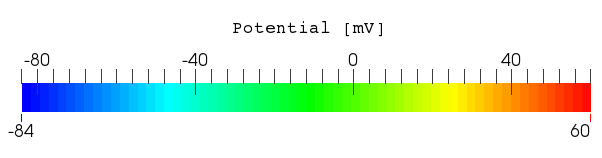
\includegraphics[height = 1.5 cm]{fig/numerical_example_mde+min_exp1_colourbar}
	} \\
\subfigure[0 ms]{
	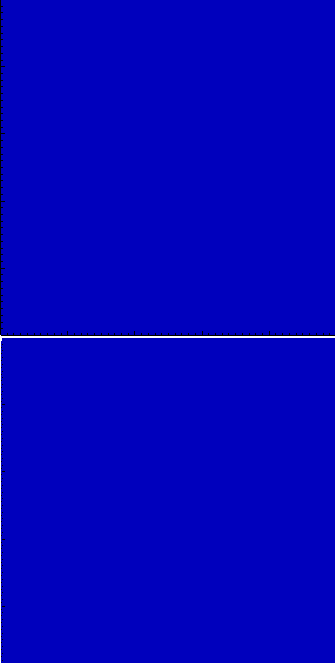
\includegraphics[height = 8 cm]{fig/numerical_example_mde+min_exp2_0ms}
	}
\subfigure[3 ms]{
	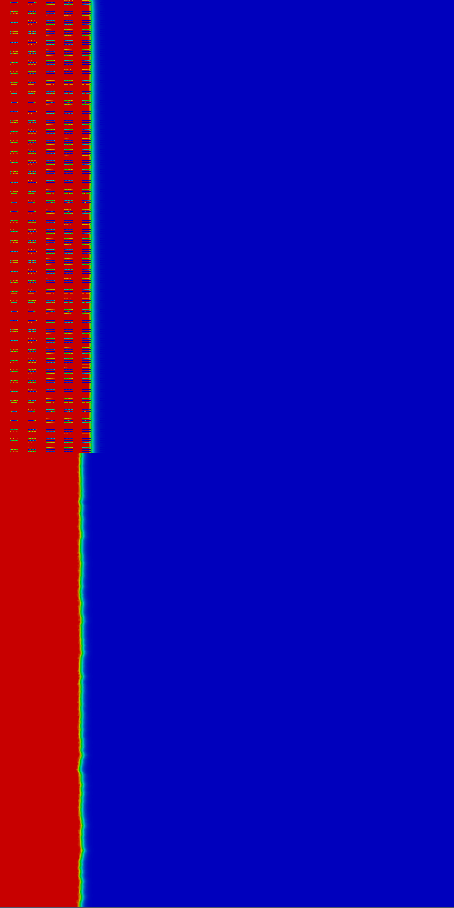
\includegraphics[height = 8 cm]{fig/numerical_example_mde+min_exp2_3ms}
	}	
\subfigure[17 ms]{
	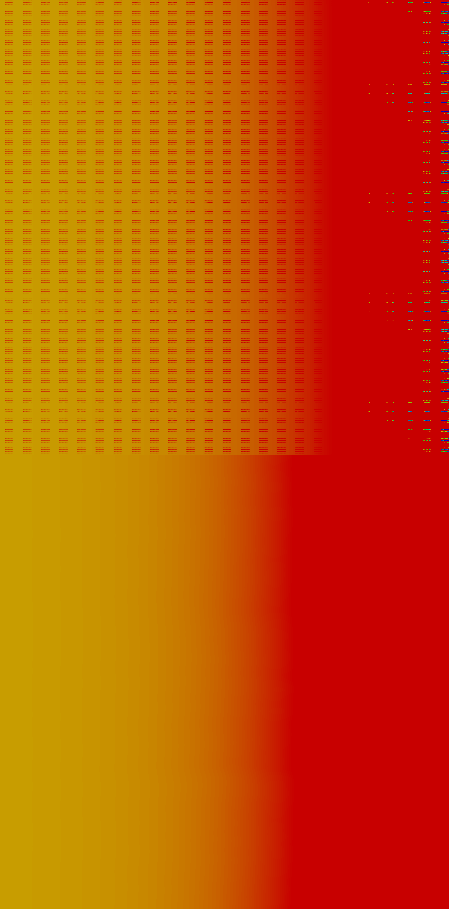
\includegraphics[height = 8 cm]{fig/numerical_example_mde+min_exp2_17ms}
	}
\subfigure[50 ms]{
	
\includegraphics[height = 8 cm]{fig/numerical_example_mde+min_exp2_50ms}
	}
\subfigure[150 ms]{
	
\includegraphics[height = 8 cm]{fig/numerical_example_mde+min_exp2_150ms}
	}
\subfigure[300 ms]{
	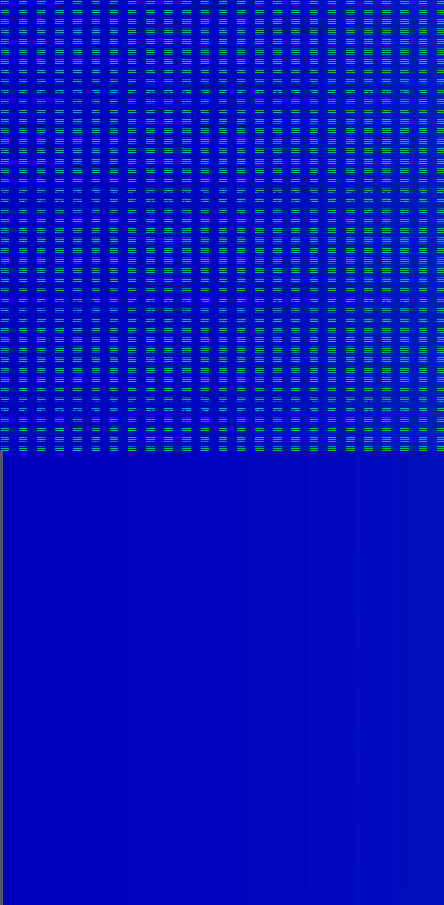
\includegraphics[height = 8 cm]{fig/numerical_example_mde+min_exp2_300ms}
	}
\subfigure[500 ms]{
	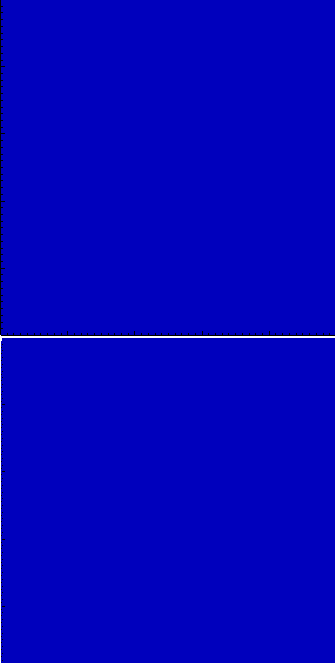
\includegraphics[height = 8 cm]{fig/numerical_example_mde+min_exp2_500ms}
	}
\caption{evolution of the potential over the tissue. The exact solution is shown up.} \label{fig:results_exp2}
\end{figure}

The relative L2-error between both, the exact and homogenized solution, stay below totally acceptable values, as can be seen in figure \ref{fig:results_exp2_error}. The  assembly times was 183.085 seconds for the exact problem, and 0.221 seconds for the homogenized one. 

\begin{figure}[H]
\centering
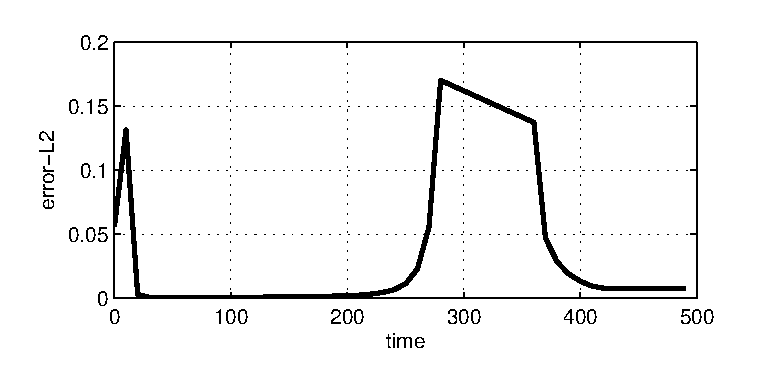
\includegraphics[height = 4 cm]{fig/numerical_example_MDE_MIN_exp2_error}
\caption{L2-error evolution between exact and homogenized problem.}
\end{figure}

In the figure \ref{fig:results_exp2_benchmark} the computing time for solve the linear system is shown. Finally, the total time, for both problem, was 7.48 hrs. The calculation was done in a 8-proccesor intel core i7 machine, with 16 gb of ram memory.

\begin{figure}[H]
\centering
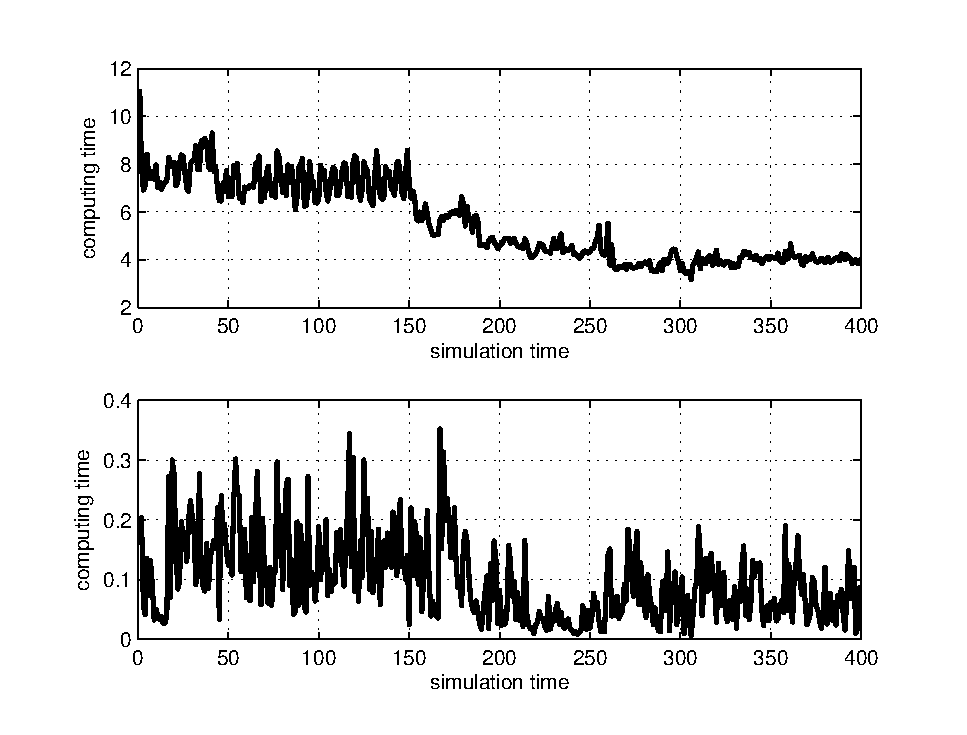
\includegraphics[height = 7 cm]{fig/numerical_example_MDE_MIN_exp2_benchmark.eps}
\caption{benchmark for experiment \# 3.} \label{fig:results_exp2_benchmark}
\end{figure}

The conduction velocities are 1.66 [mm/ms] and 1.46 [mm/ms] for the exact and the homogenized solution, respectively. The difference of the value is maybe cause the front wave propagates without obstacles in some paths for the exact solution, while the homogenized one reproduces a \textsl{medium} behaviour. A more realistic randomly distributed fibrosis would provide more similar CV values for the solutions. \\

Nevertheless, note that the results are satisfactory, cause the homogenized solution evolution reproduce the exact one in a mesoscopic scale, where relay the interest of this study. 

\newpage
\subsection{A Tissue with Vertical Walls of Fibrosis}

The configuration of the table \ref{tab:mde_min_setup_3} will be used to simulate a mid-myocardial tissue. Note that $\theta_c = 1$, so now there are vertical obstacles for the diffusion of the potential, as in figure \ref{fig:mde_min_exp2_mesh}. The reason to choose this configuration relays in impose a difficult case for the homogenization technique. The characteristic mesh sizes are the same as the previous example.

\begin{table}[H]
\centering
\begin{tabular}{@{}lr@{}}
\toprule
\multicolumn{1}{c}{Parameter} & \multicolumn{1}{c}{Set-Up}                                            \\ \midrule
Domain                        & $[0, 25] \times [0, 25] mm^2$ square                                    \\
Boundary Conditions           & $\phi = 0$, $r = 1$, $w = 1$ and $s = 0$, $\forall \vec{x} \in \Omega$ \\
Initial Conditions            & $\phi = 0$, $r = 1$, $w = 1$ and $s = 0$, $\forall \vec{x} \in \Omega$             \\
DOF's for Exact Problem       &    															 \\
DOF's for Homogenized Pb.     & 1336473                                                                   \\
$d_1$						 & 0.1171 $[mm^2/s]$  												 \\
b & 1 [mm] \\
$\theta_f$                    & 0.04                                                                   \\
$\beta$                       & $10^{-5}$                                                             \\
$\gamma$                      & 4                                                                     \\
$\Delta t $                  & 0.1 [ms]                                                                \\
Total time &	 20 [ms] \\ \bottomrule
\end{tabular}
\caption{setup for experiment.} \label{tab:mde_min_setup_3}
\end{table}

\begin{figure}[H]
\begin{center}
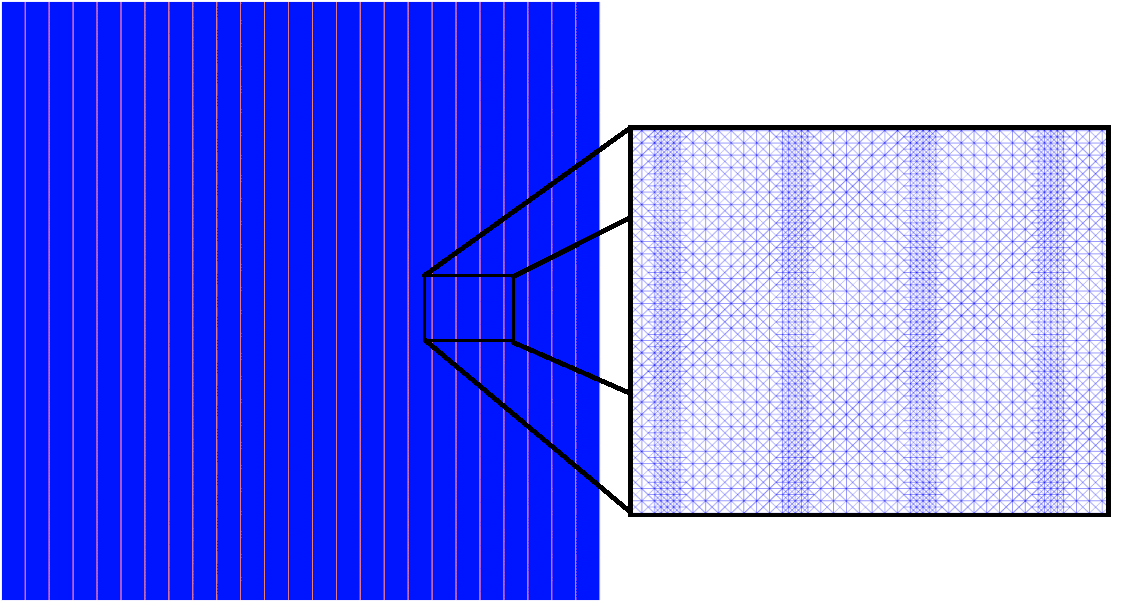
\includegraphics[height = 4.5 cm]{fig/asdasd}
\caption{ domain with vertical obstacles of callagen (left) and a zoom of the mesh used to solve the exact problem (rigth)} \label{fig:mde_min_exp2_mesh}
\end{center}
\end{figure}

The result of the implementation is presented in the figure \ref{fig:results_exp3}.

\begin{figure}[H]
\centering
\subfigure{
	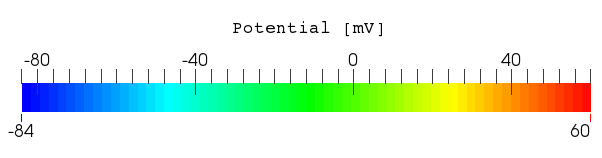
\includegraphics[height = 1.5 cm]{fig/numerical_example_mde+min_exp1_colourbar}
	} \\
\subfigure[0 ms]{
	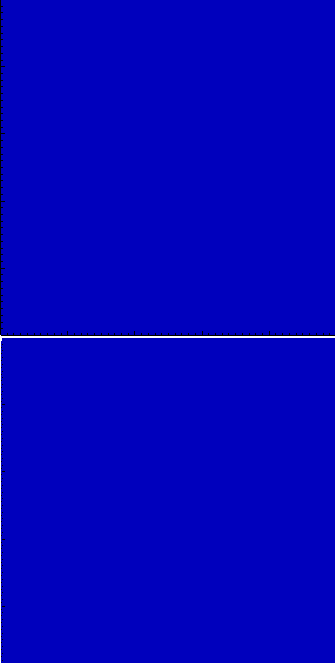
\includegraphics[height = 6 cm]{fig/numerical_example_mde+min_exp3_0ms}
	}
\subfigure[2 ms]{
	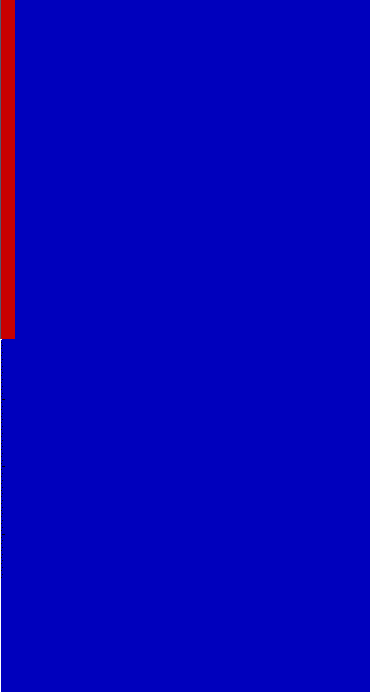
\includegraphics[height = 6 cm]{fig/numerical_example_mde+min_exp3_2ms}
	}	
\subfigure[7 ms]{
	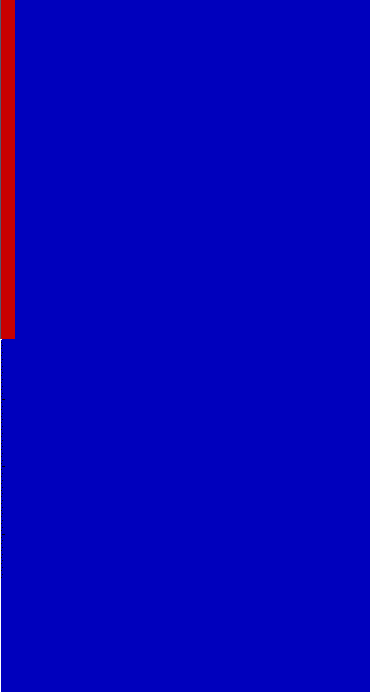
\includegraphics[height = 6 cm]{fig/numerical_example_mde+min_exp3_7ms}
	}
\subfigure[20 ms]{
	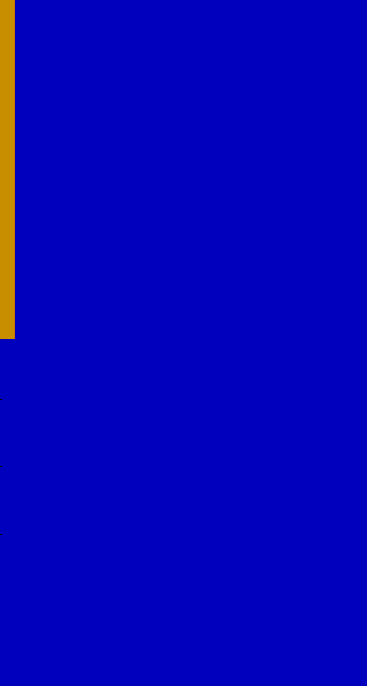
\includegraphics[height = 6 cm]{fig/numerical_example_mde+min_exp3_20ms}
	}
\caption{evolution of the potential over the tissue for the exact (up) and the homogenized (down) problem.} \label{fig:results_exp3}
\end{figure}


Note that the homogenized solution reproduce the vertical blocking the diffusion in the main fiber directions, wich is natural considering the construction of the effective tensor. So, in the scale of study, the result is satisfactory.

\newpage 
\section{Appendix 1: About the Discretization of the System of Equations (\ref{eq:mde_min})}

The time discretization of the gating variables is semi-implicit, as in the single cell experiment. So, first, for each time-step, the ODE's are solved using:


\begin{equation}
\arraycolsep=1.4pt\def\arraystretch{2.8}
\begin{array}{l}
r^{n+1} = \dfrac{r^n + (\Delta t r_{\infty}(1 - H(\phi - \theta_r)))/\tau_r^-}{1  +  (\Delta t (1 - H(\phi^n - \theta_r)))/\tau_r^- + (\Delta t H(\phi^n - \theta_r))/\tau_r^+} \\

w^{n+1} = \dfrac{w^n + (\Delta t w_{\infty}(1 - H(\phi - \theta_w)))/\tau_w^-}{1  +  (\Delta t (1 - H(\phi^n - \theta_w)))/\tau_w^- + (\Delta t H(\phi^n - \theta_w))/\tau_w^+} \\
   
s^{n+1} = \dfrac{s^n + \Delta t (1 + tanh(k_s (\phi^n - \phi_s)))/(2 \tau_s)}{(1 + \Delta t / \tau_s)}
\end{array} 
\end{equation}

in order to solve the time-discretized PDE:

\begin{equation}
\dfrac{\phi^{n + 1} - \phi^n}{\Delta t}=  div(D \nabla \phi^{n+1}) - \Delta t (J_{fi}^n + +  J_{si}^n + J_{so}^n) 
\end{equation}

So, the idea is to solve a stationary problem for each time step. This labor will be achieve trough a finite element method. \\

Let's consider the test function space $V = \{ v \in H_0^1(\Omega) \}$. Multiplying the PDE by a function of this space, integrating over all $\Omega$, considering the no-flux boundary conditions, and remembering the Green's Theorem, the weak form of the partial differential equation is obtained, so the problem can be re-written in the form $a^{n+1} (\phi^{n+1}, v) = L (v)$ as follows:

\begin{align}
a^{n+1} (\phi, v) = & \int_{\Omega} \phi v  d \Omega + \Delta t \int_{\Omega} D \nabla \phi \nabla v d \Omega \\
L (v) = & \int_{\Omega} \phi^n v d \Omega + \Delta t \int_{\Gamma_N} g v ds - \Delta t \int_{\Omega}( J_{fi}^n +  J_{si}^n + J_{so}^n )v d \Omega \label{eq:mde_min_weak}
\end{align}

where the notation $\phi = \phi^{n+1}$ is taken while there is no confusion in the meaning of the variables. Note that the currents are calculated using $\phi^n$, $r^{n+1}$, $w^{n+1}$ and $s^{n+1}$. \\

Now, lets consider the finite dimensional space $\overline{V} \subset V$ and the Galerkin method:

\begin{equation}
\phi = (c_1, c_2, ..., c_k) (\xi_1, \xi_2, ...., \xi_k)^T = \sum_{i=1}^k a_i \xi_i \label{eq:galerkin_method}
\end{equation}

where k is the total number of degrees of freedom, the functions $\{\xi_i \}_{i=1}^k$ belongs to the space $\overline{V}$ and $c_i$ is the solution at the i-node. This way, the equation (\ref{eq:mde_min_weak}) can be spatially discretized replacing (\ref{eq:galerkin_method}) on it. So, lets be $\overline{a} = \overline{L}$ the discretized weak form of the problem, then:

\begin{align*}
\overline{a} = & \int_{\Omega} (c_1, c_2, ..., c_k) (\xi_1, \xi_2, ...., \xi_k)^T (\xi_1, \xi_2, ...., \xi_k) d \Omega + \Delta t \int_{\Omega} D (c_1, c_2, ..., c_k) (\nabla \xi_1, \nabla \xi_2, ...., \nabla \xi_k)^T (\nabla \xi_1, \nabla \xi_2, ...., \nabla \xi_k) d \Omega \\
\overline{L} = & \int_{\Omega} (c_1^n, c_2^n, ..., c_k^n) (\xi_1, \xi_2, ...., \xi_k)^T (\xi_1, \xi_2, ...., \xi_k) d \Omega - \Delta t \int_{\Omega} (\gamma_1, \gamma_2, ..., \gamma_k) (\xi_1, \xi_2, ...., \xi_k)^T (\xi_1, \xi_2, ...., \xi_k) d \Omega
\end{align*}

where the test functions was discretized with functions of $\overline{V}$. The current $J^n = J_{so}^n + J_{si}^n + J_{fi}^n$ was also discretized using $J = \sum_{i=1}^k \gamma_i \xi_i$. Now, defining the usually called \textsl{mass matrix}  $M \in \mathbb{M}_{k \times k}; M_{ij} = \int \xi_i \xi_j d \Omega $ and the \textsl{stifness matrix} $K \in \mathbb{M}_{k \times k}; K_{ij} = \int \nabla \xi_i  \nabla \xi_j d \Omega$, the discretized weak form reduces to:

\begin{equation}
(M + \Delta t K) c^{n+1} = M c^n - \Delta t M \vec{\gamma} \label{eq:Ax=b}
\end{equation}

where $c^{n+1} = (c_1, c_2, ..., c_n)$ and $c^n = (c_1^n, c_2^n, ..., c_k^n)$. Finally, the space $\overline{V}$ is chosen as the set of $\mathbb{P}_1$-Lagrange functions.

\begin{figure}[H]
\centering
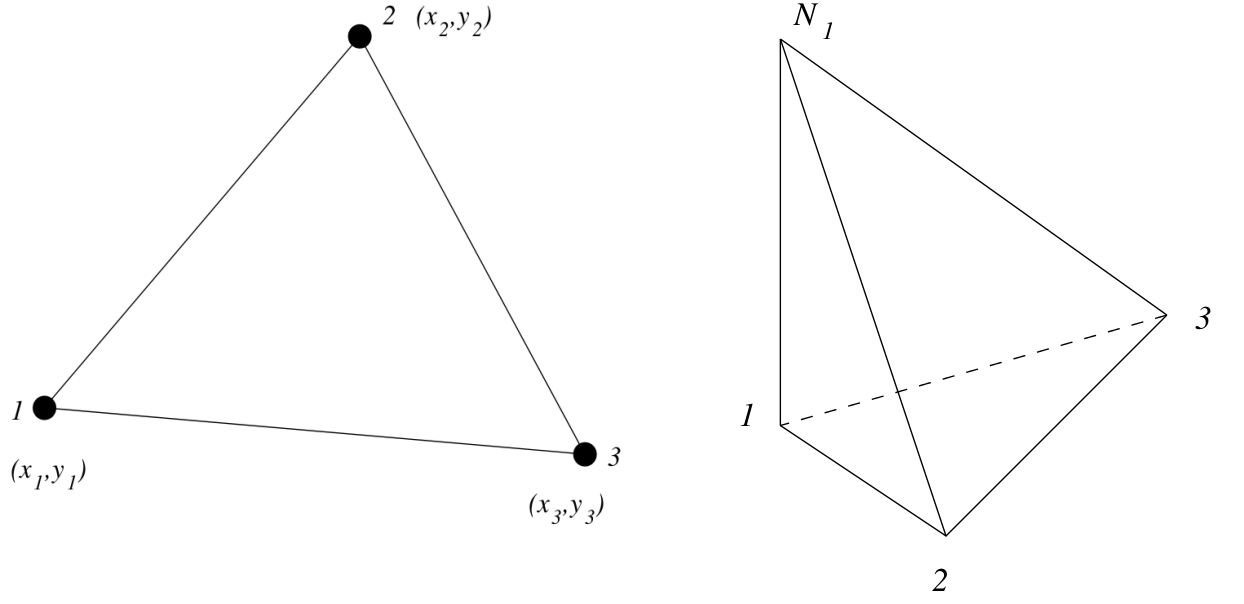
\includegraphics[height = 5 cm]{fig/fem_p1_shape_functions}
\caption{$\mathbb{P}_1$-Lagrange triangle basis example.}
\end{figure}

Now, to solve the linear system (\ref{eq:Ax=b}) two methods, accordingly to the number of DOF's of the problem will be used:

\begin{itemize}
\item AMG preconditioner $+$ conjugate gradiente ($\# DOF's > 200.000$): for large systems, like the obtained for the exact problem with diffuse fibrosis, an algebraic multigrid preconditioner is applied, followed by the conjugate gradient iterative method.
\item Gaussian elimination ($\# DOF's < 200.000$): this direct method is used for relatively small systems, like the one obtained for the homogenized problem.
\end{itemize}

The update of the \textsl{rhs} vector $(M c^n - \Delta t M \vec{\gamma})$ and the resolution of the linear problem is done at each time-step, while the matrix $(M + \Delta t K)$ is just assembled once at the start.

\newpage
\section{About the conduction Velocity}

$\theta_c = 0   \rightarrow 1.389 ~ mm/ms$ \\
$\theta_c = 0.4 \rightarrow 0.953 ~ mm/ms$

\newpage
\section{Randomly generated fibrosis}

On this section the same problem will be solved but using a randmoly distributed diffuse fibrosis, as in the Panfilov's results (todo: citar!), in order to compare different phenomena, as the effect of the fibrosis in the conduction velocity, the generation of the spiral waves, and the spiral break-up. 

\newpage
\section{A Litle comparison of Solution methods}

A 25x25 mesh of nearly 80000 dof is considered for exact problem and a 50000 dof mesh for the homogenized problem. The first 20 ms of the simulations takes:

\begin{itemize}
\item Set-up 1: EP: cg/amg, save factorization for amg, non zero guess. HP: LU direct solver.
\begin{itemize}
\item serial: 17.32 (seg)
\item parallel: 9.56 (seg)
\end{itemize}
\item Set-up 2: EP: cg + amg, HP: LU direct solver.
\begin{itemize}
\item serial: 22.27 (seg)
\item parallel: 12.087 (seg)
\end{itemize}
\item Set-up 3: EP: cg + icc, HP: LU direct solver.
\begin{itemize}
\item serial: 13.22 (seg)
\item parallel: --
\end{itemize}
\end{itemize}